% This is based on the LLNCS.DEM the demonstration file of
% the LaTeX macro package from Springer-Verlag
% for Lecture Notes in Computer Science,
% version 2.4 for LaTeX2e as of 16. April 2010
%
% See http://www.springer.com/computer/lncs/lncs+authors?SGWID=0-40209-0-0-0
% for the full guidelines.
%
\documentclass{llncs}
\usepackage{tikz}
\usepackage{pgfplots}
\usepackage{algorithm2e}
\usepackage{listings}
\usepackage{color}
\usepackage{hyperref}
\usepackage{geometry}
\geometry{
  a4paper,         % or letterpaper
  textwidth=15cm,  % llncs has 12.2cm
  textheight=24cm, % llncs has 19.3cm
  heightrounded,   % integer number of lines
  hratio=1:1,      % horizontally centered
  vratio=2:3,      % not vertically centered
}

\definecolor{dkgreen}{rgb}{0,0.6,0}
\definecolor{gray}{rgb}{0.5,0.5,0.5}
\definecolor{mauve}{rgb}{0.58,0,0.82}

\lstset{frame=tb,
  language=Java,
  aboveskip=3mm,
  belowskip=3mm,
  showstringspaces=false,
  columns=flexible,
  basicstyle={\small\ttfamily},
  numbers=none,
  numberstyle=\tiny\color{gray},
  keywordstyle=\color{blue},
  commentstyle=\color{dkgreen},
  stringstyle=\color{mauve},
  breaklines=true,
  breakatwhitespace=true,
  tabsize=3
}
\begin{document}


\title{Algor\'{i}tmica II. Algoritmos Metaheur\'{i}sticos}
%
\titlerunning{Enfriamiento Simulado}  % abbreviated title (for running head)
%                                     also used for the TOC unless
%                                     \toctitle is used
%
\author{Joaq\'{i}n Roiz Pagador\inst{1}}
%
\authorrunning{Ivar Ekeland et al.} % abbreviated author list (for running head)
%
%
\institute{Universidad Pablo de Olavide, Carretera Utrera s/n, Sevilla, Espa\~{n}a,\\
\email{quiniroiz@gmail.com}}

\maketitle              % typeset the title of the contribution

\begin{abstract}
El siguiente documento pertenece a una serie de documentos que pretende servir a modo de res\'{u}men para el temario de Algor\'{i}tmica II para el Grado en Ingenier\'{i}a Inform\'{a}tica en Sistemas de Informaci\'{o}n.\\
\keywords{algoritmos, metaheur\'{i}stica, b\'{u}squeda, tab\'{u}}
\end{abstract}
%
\section*{B\'{u}squeda Tab\'{u}.}
%
El algoritmo de b\'{u}squeda tab\'{u} fue propuesto por Glover en 1986. En 1990, este algoritmo lleg\'{o} a ser muy popular solventando problemas de optimizaci\'{o}n de forma aproximada. Hoy en d\'{i}a es uno de los algoritmos metaheur\'{i}sticos m\'{a}s extendidos.\\

Comparando con el enfriamiento simulado,  podemos observar que esta t\'{e}cnica es menos aleatoria, TS acepta peores movimientos y modifica entornos. Tambi\'{e}n utiliza la memoria adaptativa y estrategias especiales de resoluci\'{o}n de problemas.\\

Principales ventajas de TS:\\
\begin{enumerate}
\item Restringe el entorno de b\'{u}squeda.
\begin{itemize}
\item Evitamos recorridos C\'{i}clicos.
\item Generamos vecinos modificados.
\end{itemize}
\item Introducimos mecanismos de reinicializaci\'{o}n.
\begin{itemize}
\item Intensificamos en zonas exploradas.
\item Diversificamos en zonas poco visitadas.
\end{itemize}
\end{enumerate}

Se utilizar\'{a}n dos tipos de memoria:
\begin{enumerate}
\item Memorias a corto plazo o lista tab\'{u} $\gets$ Decisi\'{o}n de vecinos. Guarda informaci\'{o}n que permite guiar la b\'{u}squeda de forma inmediata, desde el comienzo del procedimiento (entornos restringidos/tab\'{u})
\item Memorias a largo plazo $\gets$ B\'{u}squeda de nuevo m\'{a}ximo. Guarda informaci\'{o}n que permite guiar la b\'{u}squeda a \textit{posteriori}, despu\'{e}s de una primera etapa en la que se han realizado una o varias ejecuciones del algoritmo aplicando la memoria a corto plazo.
\end{enumerate}

\textit{La lista ser\'{a} din\'{a}mica, es decir, habr\'{a} cambios.}\\

El principio de TS podr\'{i}a resumirse como: ''Es mejor una mala decisi\'{o}n basada en informaci\'{o}n que una buena decisi\'{o}n al azar, ya que, en un sistema que emplea memoria, una mala elecci\'{o}n basada en una estraategia proporcionar\'{a} claves \'{u}tiles para continuar la b\'{u}squeda. Una buena elecci\'{o}n fruto del azar no proporcionar\'{a} ninguna informaci\'{o}n para posteriores acciones.'' (F.Glover)\\

\begin{center}
\textbf{Memoria $+$ Aprendizaje $=$ B\'{u}squeda inteligente}
\end{center}

TS expl\'{i}citamente usa el historial de b\'{u}squeda. Aplica una b\'{u}squeda local y usa una memoria a corto plazo para escapar del m\'{i}nimo local y evitar ciclos. La memoria a corto plazo implementa una lista tab\'{u} que almacenar\'{a} un listado de vecinos visitados con soluciones y proh\'{i}be utilizarlas nuevamente.\\

En los siguientes puntos describiremos las memorias a corto y a largo plazo, pero a groso modo podemos decir que, por cada iteraci\'{o}n en la lista tab\'{u}, a modo de cola de prioridades, un elemento se insertar\'{a}, y el m\'{a}s antiguo se eliminar\'{a}, similar a un sistema FIFO.\\

El algoritmo parar\'{a} cuando una condici\'{o}n de parada es encontrada, por ejemplo, cuando el n\'{u}mero de soluciones prohibidas en la lista tab\'{u} es completo.\\

Una lista tab\'{u} de tama\~{n}o peque\~{n}o har\'{a} que se concentre la b\'{u}squeda en peque\~{n}as \'{a}reas del espacio de b\'{u}squeda. Por el contrario, una lista tab\'{u} de mayor tama\~'{n}o fuerza el proceso de b\'{u}squedas en regiones m\'{a}s extensas, debido a que \'{e}sto proh\'{i}be revisitar un alto n\'{u}mero de soluciones.\\ 

\subsection*{Memoria a Corto Plazo}
\begin{itemize}
\item Modificaci\'{o}n de las estructuras de entorno.
\begin{itemize}
\item La TS restringe la b\'{u}squeda local sustituyendo E($S_{act}$) por otro entorno E*($S_{act}$). En cada iteraci\'{o}n, se acepta siempre el mejor vecino de dicho entorno, tanto si es peor como si es mejor que $S_{act}$.
\item La memoria de corto placo (\textbf{Lista tab\'{u}}) permite a la TS determinar E*($S_{act}$) y as\'{i} organizar la manera en la que se explora el espacio.
\end{itemize}
\item Las soluciones admitidas en E*($S_{act}$) dependen d ela estructura de la lista tab\'{u}:
\begin{itemize}
\item \textbf{Lista de soluciones tab\'{u}}. Soluciones ya visitadas que se marcan como tab\'{u} para no volver a ellas, elimin\'{a}ndolas del vecindario de $S_{act}$.
\item \textbf{Lista de movimientos tab\'{u}}. Se eliminan del entorno todos los vecinos resultantes de aplicar sobre $S_{act}$ un movimiento realizado anteriormente.
\item \textbf{Lista de valores de atributos tab\'{u}}. Se eliminan del entorno todos aquellos vecinos con un par (atributo, valor) determinado que ya presentara alguna soluci\'{o}n explorada anteriormente (NOTA: en TSP no nos vendr\'{i}a bien, mejor dependencias como d\'{i}a, clima, tr\'{a}fico...).
\end{itemize}
\item Tendencia tab\'{u}. Tiempo que una soluci\'{o}n permanece en la lista tab\'{u}.
\item Niveles de aspirraci\'{o}n: Introduce flexibilidad.
\begin{itemize}
\item Se genera una soluci\'{o}n mejor que cualquiera anterior.
\item Se alcanza valor aceptable.
\item Se alcanza el mejor valor conocido.
\end{itemize}
\item Estrategias para listas de candidatos.
\begin{itemize}
\item Restringen el n\'{u}mero de vecinos examinados en una iteraci\'{o}n dada, para los casos en los que E*($S_{act}$) es grande o la evaluaci\'{o}n costosa.
\item Se busca el mejor movimiento disponible que pueda ser determinado con esfuerzo equilibrado.
\item Se genera una parte del espacio y se toma el mejor vecino.
\end{itemize}
\end{itemize}

Una selecci\'{o}n adecuada puede reducir el Tiempo Computacional.

\subsection*{Memoria a Largo Plazo}
En algunas aplicaciones, las componentes de la memoria TS de corto plazo son suficientes para producir soluciones de muy alta calidad. Pero TS se vuelve mucho m\'{a}s potente incluyendo memoria de largo plazo. La memoria de largo plazo se puede usar de dos modos:\\
\begin{itemize}
\item Intensificaci\'{o}n y diversificaci\'{o}n. Memoria de frecuencias y visitas a una soluci\'{o}n.
\item Reinicializar la b\'{u}squeda, mantener registro de mejores soluciones.. Se pueden usar para diversificar.
\item Flowchart $\rightarrow$ Serie de iteraciones a corto plazo, donde extraemos la mejor de ellas.
\item Nueva soluci\'{o}n a partir de lo almacenado, evitaremos repetir.
\end{itemize}

Una estructura muy empleada es la memoria de frecuencias, que registra el n\'{u}mero de veces que cada valor de un atributo ha pertenecido a soluciones visitadas en la b\'{u}squeda.

\subsubsection{Estrategias de Intensificaci\'{o}n}
\begin{itemize}
\item Se basan en una reinicializaci\'{o}n de la b\'{u}squeda que efect\'{u}a un regreso a regiones atractivas del espacio para buscar en ellas m\'{a}s extensamente.
\item Se mantiene un registro de las mejores soluciones visitadas, insertando una nueva soluci\'{o}n cada vez que se convierte en la mejor.
\item Se puede introducir una medida de diversificaci\'{o}n para asegurar que las soluciones registradas difieran una de otra en un grado deseado.
\end{itemize}


\begin{figure}[h]
\centering
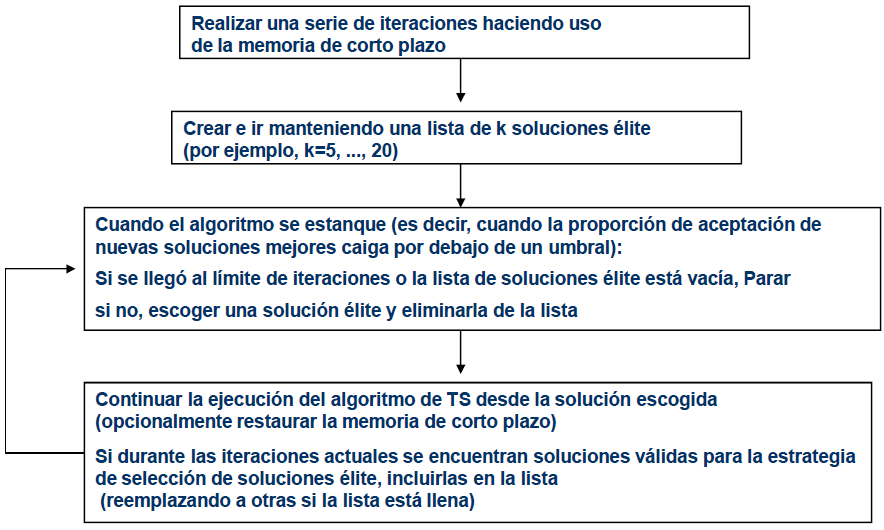
\includegraphics[scale=0.7]{img/intensificacion.png}
\caption{Flowchart Intensificaci\'{o}n}
\end{figure}

\subsubsection{Estrategias de Diversificaci\'{o}n}
\begin{itemize}
\item Conducen la b\'{u}squeda hacia nuevas regiones del espacio de b\'{u}squeda no exploradas a\'{u}n.
\item La b\'{u}squeda se reinicializa cuando se estanca, partiendo de una soluci\'{o}n no visitada.
\item Esta soluci\'{o}n se genera a partir de la memoria de frecuencias, dando mayor probabilidad de aparici\'{o}n a los valores menor habituales.


\begin{figure}[h]
\centering
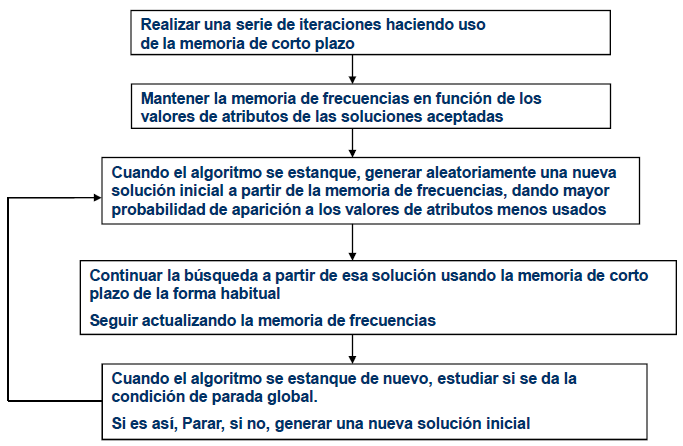
\includegraphics[scale=0.9]{img/diversificacion.png}
\caption{Flowchart Diversificaci\'{o}n}
\end{figure}
\end{itemize}

\subsubsection{Estructuras de memoria largo plazo}
\begin{itemize}
\item Si las variables son binarias, se puede usar un vector de dimensi\'{o}n n, para almacenar el n\'{u}mero de veces que cada variable tom\'{o} el valor 0 (\'{o} 1).
\item Si son enteras, se utiliza una matriz bidimensional, como contador de las veces que la variable i toma el valor k: m[i,k].
\item Si son permutaciones de orden, se puede utilizar una matriz bidimensional, como contador de las veces que el valor i ha ido seguido de j: M[i,j]
\end{itemize}

\subsubsection{Uso de las memorias de frecuencias}
\begin{enumerate}
\item Generar directamente la nueva soluci\'{o}n inicial a partir de la informaci\'{o}n almacenada en la memoria de frecuencias M, dando mayor probabilidad de aparici\'{o}n a los valores menos habituales.
\item Usar la informaci\'{o}n almacenada en M para modificar temporalmente el caso del problema, potenciando los valores heur\'{i}sticos de los atributos menos usados en la b\'{u}squeda. Aplicar un algoritmo greedy sobre ese caso modificado para generar la soluci\'{o}n inicial. Restaurar el caso original del problema antes de continuar con la b\'{u}squeda.
\end{enumerate}

\begin{figure}[h]
\centering
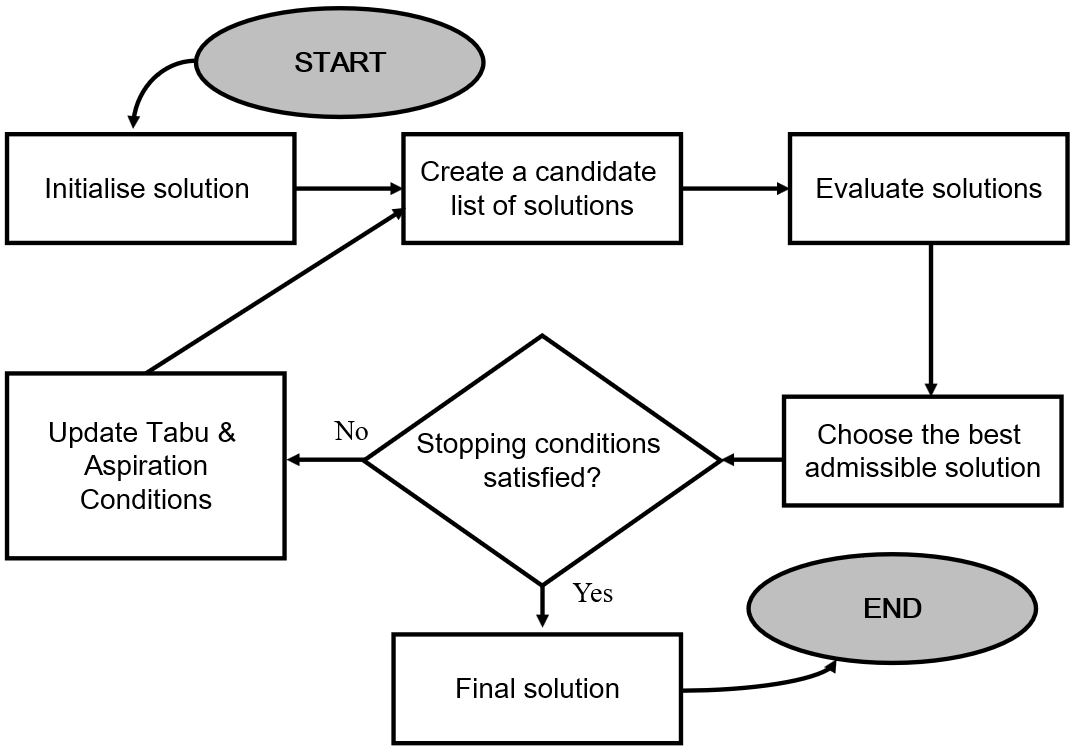
\includegraphics[scale=0.6]{img/flujo.png}
\caption{Diagrama de flujo B\'{u}squeda Tab\'{u}}
\end{figure}


\begin{algorithm}[H]
\SetKwInOut{Output}{output}
\SetKwRepeat{Do}{do}{while}
	$sBest \gets s_0$\\
    $tabuList \gets []$\\
	\While{$not stoppingCondition()$}{
	$canidateList \gets []$\\
	$bestCandidate \gets null$\\
	\For{$sCandidate in sNeightborhood$}{
		\If{$(not tabuList.contains(sCandidate)) and (fitness(sCandidate) > fitness(bestCandidate))$}{
			$bestCandidate \gets sCandidate$\\		
		}
	}
	\If{$fitness(bestCandidate) > fitness(sBest)$}
	{
		$sBest \gets bestCandidate$\\
	}
	$tabuList.push(bestCandidate)$\\
	\If{$tabuList.size > maxTabuSize$}
	{
		$tabuList.removeFist()$
	}
	}
    \Output{Best Solution found.}
    \caption{Algoritmo de B\'{u}squeda Tab\'{u} con memoria a corto plazo.}
\end{algorithm}

Si quisi\'{e}ramos a\~{n}adir una condici\'{o}n de aspiraci\'{o}n, en la condici\'{o}n perteneciente a la iteraci\'{o}n de los vecinos deber\'{i}amos a\~{n}adir ''or sCandidate.isAspiration()''.

Aplicaci\'{o}n de temario: \url{http://leeds-faculty.colorado.edu/glover/fred\%20pubs/329\%20-\%20Introduccion\%20a\%20la\%20Busqueda\%20Tabu\%20TS_Spanish\%20w\%20Belen(11-9-06).pdf}

%
% ---- Bibliography ----
%
\begin{thebibliography}{5}

\bibitem{UGR}
  Material asignatura,
  \textit{Metaheur\'{i}sticas},
  UGR. \url{http://sci2s.ugr.es/graduateCourses/Metaheuristicas}
\bibitem{libro}
  E.-G. Talbi, Metaheuristics. From design to implementation,
  Wiley, 2009 Material.
\bibitem{folleto}
	C. Blum, A Roli, Metaheuristics in Combinatorial Optimization: overview and conceptual comparison. ACM Computing Surveys, 35(3), 2003, 268-308.
	\bibitem{ampliacion}
	B. Meli\'{a}n, F. Glover. Introducci\'{o}n a la b\'{u}queda tab\'{u}, 2006. \url{http://leeds-faculty.colorado.edu/glover/fred\%20pubs/329\%20-\%20Introduccion\%20a\%20la\%20Busqueda\%20Tabu\%20TS_Spanish\%20w\%20Belen(11-9-06).pdf}
 

\end{thebibliography}

\end{document}
